\section{Hardware}
\label{sec:hw}

In this section hardware used in the process of creating capture device is described.
\todo[inline]{dlhsi text}

\subsection{Hardware Setup}
To be able to effectively scan 2d biometry of hand various hardware is necessary. Firstly we need structure to hold all other
hardware together robust enought to hold weight and absorb vibrations generated by rail. This need is satisfied by using aluminium framework.
Rail itself is mounted in this framework in a way to allow slide to move freely above the hand position. Camera and light are mounted on the slide
moving along the rail to allow continuous capture of hand geometry with best lightning conditions.
Control module consists from controllers running software necessary for capturing hand geometry.
\begin{figure}[ht!]
    \label{fig:setup}
    \centering
    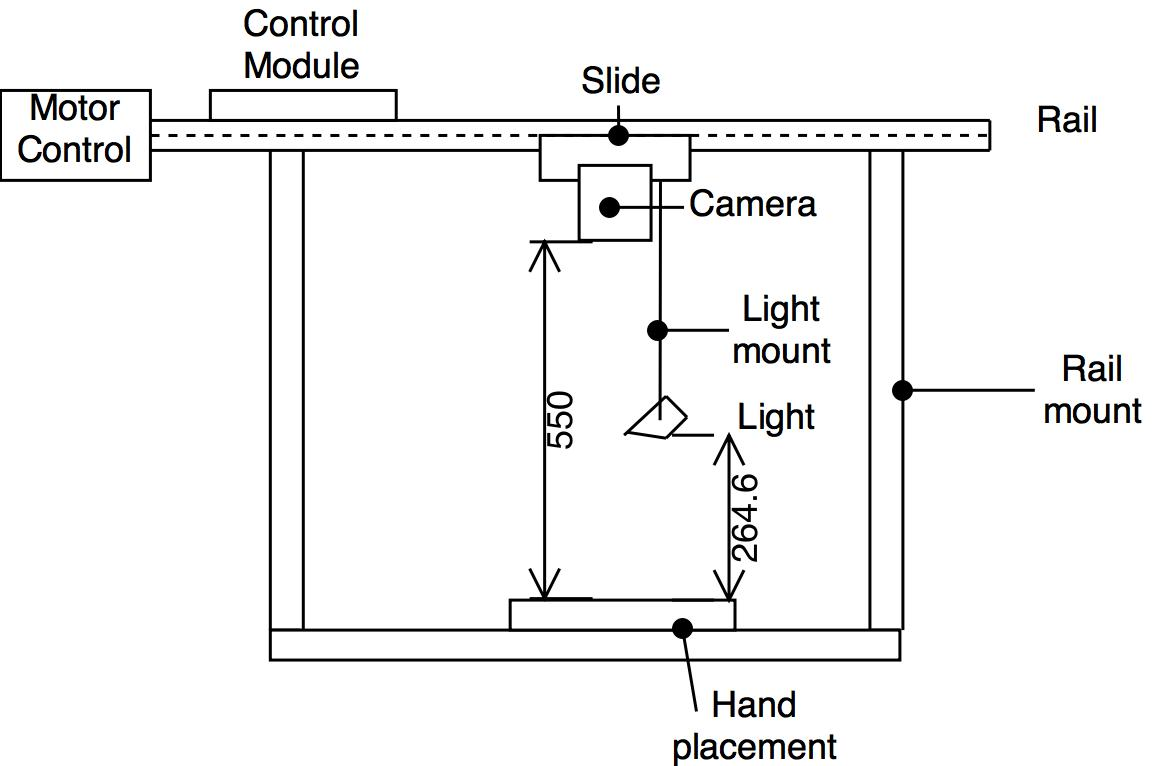
\includegraphics[width=0.75\linewidth]{setup.jpg}
    \caption{Schematic of hardware setup.}
\end{figure}

%\begin{figure}[ht]
%    \label{fig:overview}
%    \centering
%    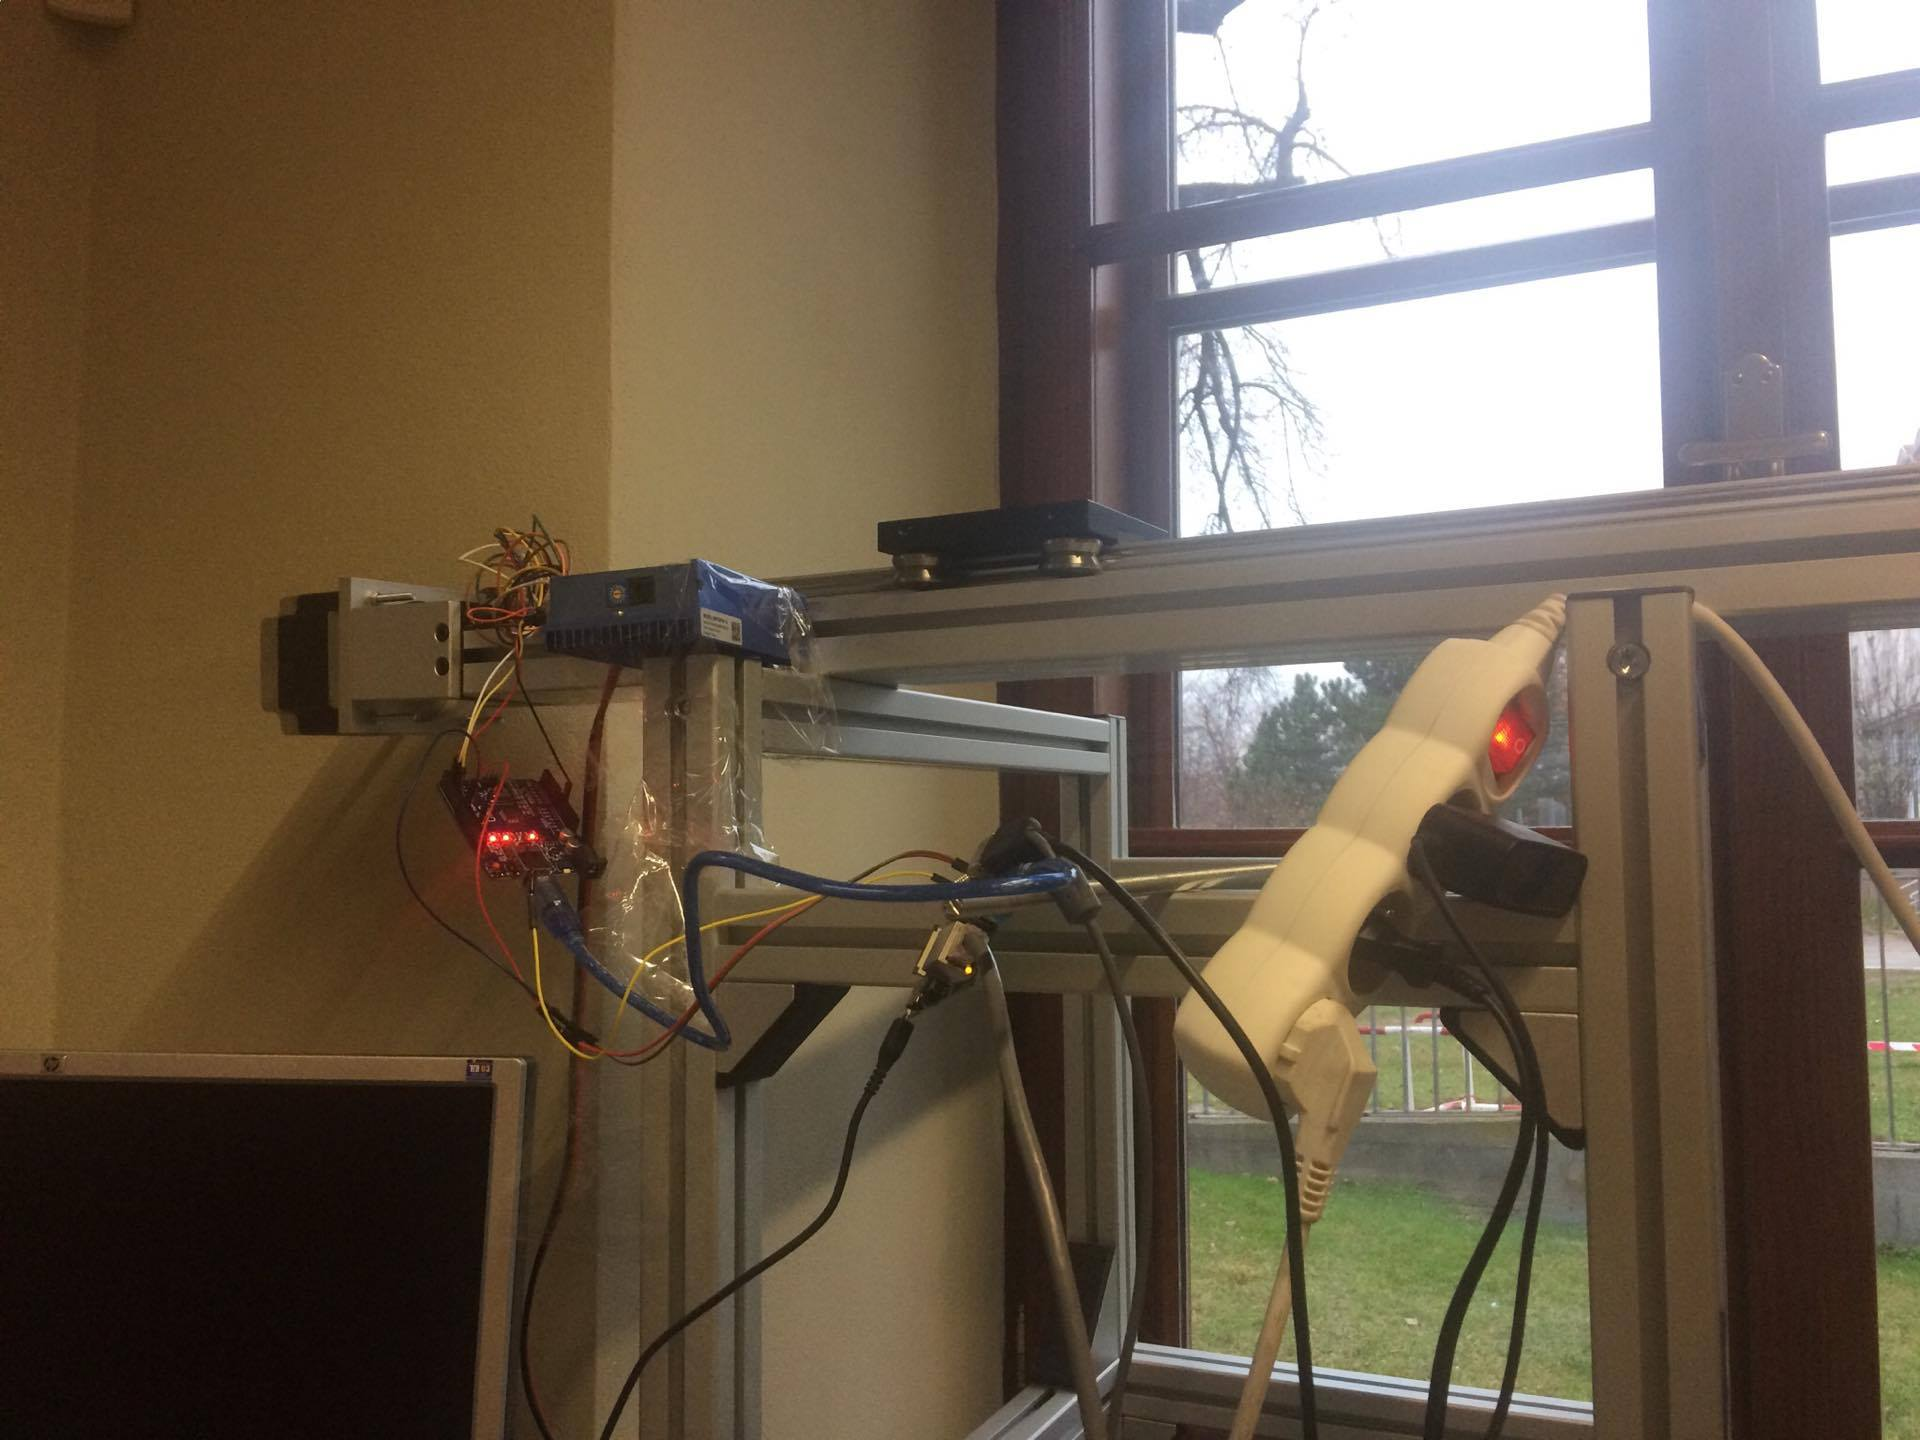
\includegraphics[width=0.75\linewidth]{overview.jpg}
%    \caption{Hardware Setup.}
%    \todo[inline]{nova foto}
%\end{figure}

\subsubsection*{Camera}
The selected camera is Basler raL6144-16gm. This camera provides us with the resolution of 6144 $\times$ 1 pixels with line rate up to 17 kHz.
The captured image is in greyscale colors which is the desired output for our usecase. The camera's shutter can be operated either via hardware
or software trigger\footnote{The camera also enables "free-run mode".}.

The camera is equipped with AF Nikkor 50mm f1.8D lens. The lens suits our needs for multiple reasons:
It is relatively inexpensive, simple to use and has good depth-of-field control with aperture ranging from f/1.8 up to f/22.

\subsubsection*{Camera Mount}
In order to acquire images with line camera either scanned object or camera have to move in smooth direct line to cover whole scan area.
We decided to move the camera because of trivial reason: to minimize errors during scaning. Hand is placed on stable platform and with only camera mount moving,
human error is minimized and user experience is improved.

Slide moving along the rail houses platform where camera is mounted. This platform is facing down with camera and light mounted as seen in figure \ref{fig:camera-mount}.

\begin{figure}[ht]
    \label{fig:camera-mount}
    \centering
    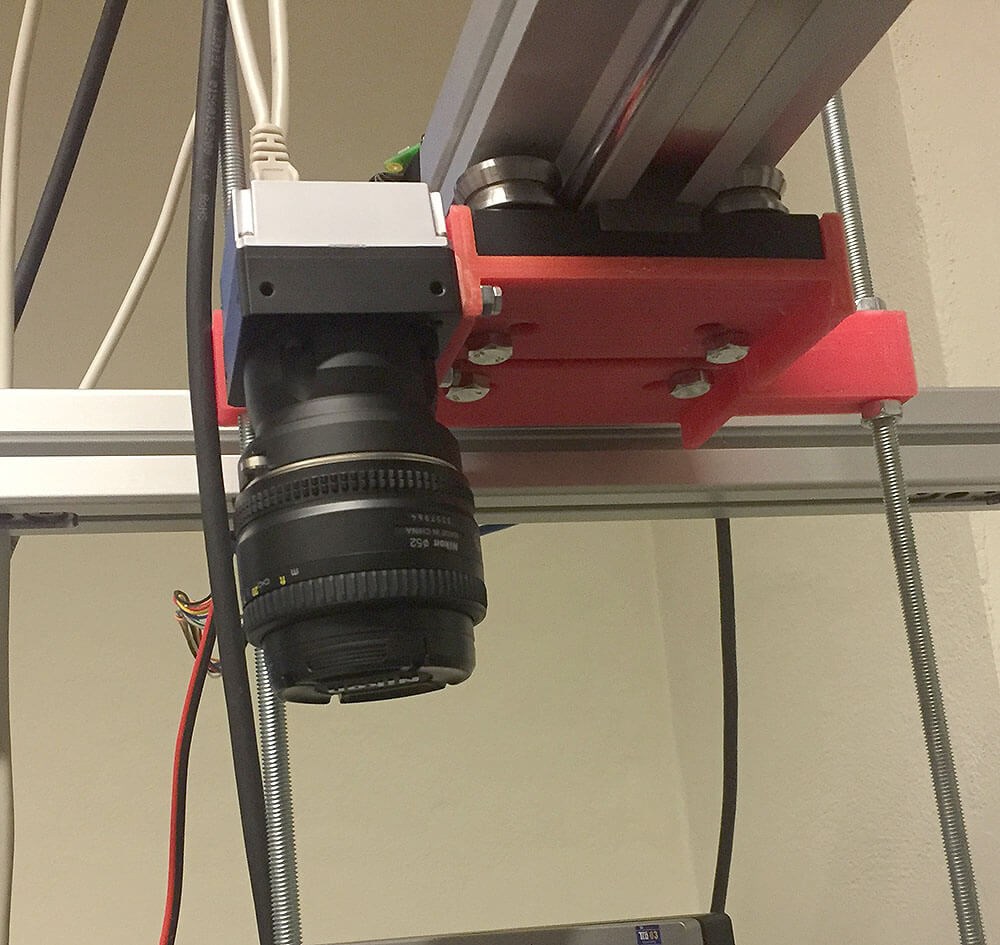
\includegraphics[width=0.5\linewidth]{camera-mount.jpg}
    \caption{camera mount setup}
\end{figure}


\subsubsection*{Slide Rail \& Stepper Motor}
Slide moves on the rail in uniform motion along rail axis. Slide movement is controlled by a stepper motorwhich controls direction and speed of the movement.
Rail is mounted on the framework in specified height calculated from camera and light focus.
\todo[inline]{Preco je to v danej vyske, vypocet vysky}

The stepper motor itself is controlled by Leadshine EM705 Digital Stepper Drive which is controlled by pulse width modulation
generated by Arduino UNO with our custom code generating 976 Hz PWM with 50\% duty cycle.
\todo[inline]{skontrolovat cisla}

The PWM can be calculated as follows:

${PWM}_{Frequency} = 16000000 / (Prescale\_Factor * 256)$

where $Prescale\_Factor$ can be set to 1, 8, 64, 256 or 1024. The default value is 64 which results in aforementioned 976 Hz PWM.

\subsection{Slide Rail Control}
Program control running on Raspberry PI 3.
The stepper motor's speed is controlled by the PWM generated on Arduino UNO providing 5V through GPIO
\footnote{When stepper motor is controlled directly from Raspberry 3.3V are insufficient and stuttering occurs.}.
Direction and \texttt{ENABLE} state are controlled through software control from Arduino UNO.
\todo[inline]{Here should be the calculation of speed}

\subsection{Light}
To acquire high precision images of hand it is necessary to have proper light source. Light is mounted directly below the slide platform
angled towards camera axis. Light used is Corona II line scan light
providing ability to illuminate currently scanned region of hand with bright light. Without this light images would be very
dark, whereas after light integration images became very clear.

Light is controlled through the RS232 interface on control unit XLC4 connected to Raspberry Pi control module.

\todo[inline]{light intensity  light.cmd("IY E 1200") }
\noindent RS232 Interface is configured as follows:
\begin{description}
    \item[Serial Port] COM4
    \item[Baudrate] 115200
    \item[Databits] 8
    \item[Stop Bits] 1
    \item[Parity] None
\end{description}

\subsection{Hand Placement}
The hand is placed in the centre of the framework on a prepared platform which aligns and spreads the fingers in order to
capture the same hand geometry during different scans. The hand is stable during image capture procedure which minimizes human error.
Figure \ref{fig:hand-placement} shows placement of hand during scan.

\begin{figure}[ht]
    \label{fig:hand-placement}
    \centering
    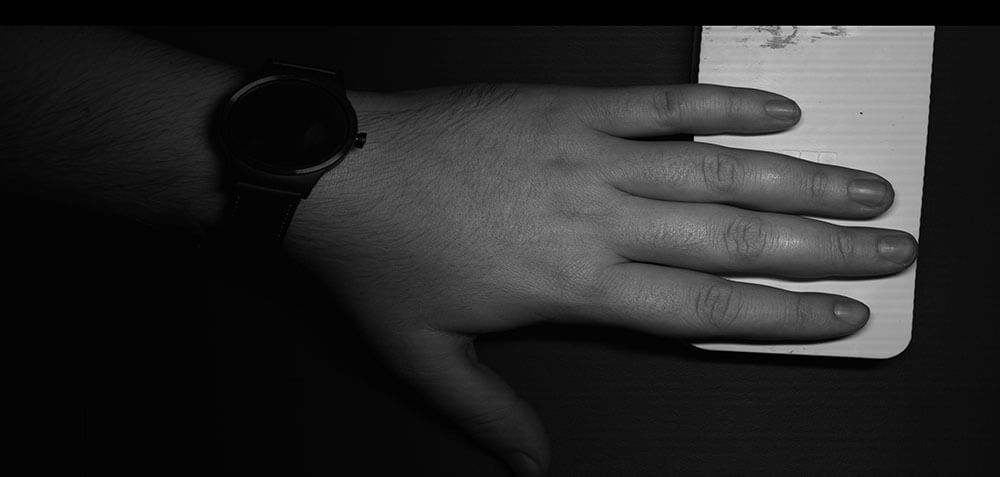
\includegraphics[width=0.8\linewidth]{hand-top.jpg}
    \caption{Hand placement during scan}
    \todo[inline]{zmenit/orezat foto}
\end{figure}

\subsection{Control module}
Control module - Raspberry Pi connects all of the hardware parts and runs software necessary for control of other parts. To control
rail slide Arduino Uno is utilizied because of neccesity for output voltage of 5V of its GPIO.
\todo[inline]{Schema zapojenia pi}

